
\section{Topología}

\begin{definicion}
    Sea $X\neq \varnothing$. Una clase $\tau$ de subconjunto de $X$ es una topología sobre $X$, se cumple: 
    \begin{enumerate}
        \item $\varnothing,X\in \tau$
        \item La unión de una clase arbitraria de conjuntos en $\tau$ es un miembro de $\tau$. 
        \item La intersección de una clase finita de miembros de $\tau$ está en $\tau$. 
    \end{enumerate}
    Los miembros de $\tau$ son los abiertos de $X$. 
\end{definicion}

\begin{cajita}
    \begin{enumerate}
        \item El par $(X,\tau)\footnotetext{estructura topológica}$ es un espacio topológico. 
        \item A los elementos de $X$ se les llama puntos. 
    \end{enumerate}
\end{cajita}

\begin{ejemplo}
    \begin{enumerate}
        \item Sea $X\neq \varnothing\implies \tau=P(X)$ es una topología sobre $X$. A $\tau$ se le llama topología discreta de $X$, y $(X,\tau)$ es un espacio discreto. 

        \item Sea $X\neq \varnothing\implies \tau =\{\varnothing,X\}$ es una topología sobre $X$. A $\tau$ se le llama topología indiscreta, y $(X,\tau)$ es un espacio indiscreto. 
        \item $X=\mathbb{R}^2$ y $\tau$ es la colección de abiertos de $\mathbb{R}^2$ definido en términos de la métrica usual. A $\tau$ se le llama topología usual de $\mathbb{R}^2$. 
        \item Sea $X=\{a,b,c,d,e\}$.
        \begin{enumerate}
            \item Sea $\tau_1=\{X,\varnothing,\{a\},\{c,d\},\{a,c,d\},\{b,c,d,e\}\}\implies \tau_1$ es una topología sobre $X$.
            \item Sea $\tau_2=\{X,\varnothing,\{a\},\{c,d\},\{a,c,d\},\{b,c,d\}\}$. Note que $\{a\}\cup \{b,c,d\}=\{a,b,c,d\}\not\in \tau_2\implies \tau_2$ no es topología sobre $X$
            \item Sea $X$ un conjunto infinito y sea $\tau$ el vacío junto con la colección de subconjunto de $X$ cuyos complementos son finitos. $\tau$ es una topología sobre $X$, y se llama topología cofinita sobre $X$. 
        \end{enumerate}  
    \end{enumerate}
\end{ejemplo}

\begin{cajita}
    \begin{nota}
        Un espacio metrizable es un espacio topológico $X$ con la propiedad que existe una métrica que genera los abiertos de la topología dada. 
    \end{nota}
    \begin{problema}
        ¿Qué tipos de espacios topológicos son metrizables?
    \end{problema}
\end{cajita}

\begin{prop}
    Si $\tau_1$ y $\tau_2$ son topologías sobre $X$, entonces $\tau_1\cap \tau_2$ es topología sobre $X$.
    \begin{dem}
        \begin{enumerate}
            \item Como $\tau_1$ y $\tau_2$ son topologías, etnonces: $X,\varnothing\in \tau_1$ y $X,\varnothing\in \tau_2\implies X\in \tau_1\cap \tau_2$ y $\varnothing\in \tau_1\cap \tau_2$. 
            \item Sea $\{G_i\}_{i\in I}$ una subcolección de $\tau_1\cap \tau_2\implies G_i\in \tau_1,\forall i\in I \implies \bigcup_i G_i\in \tau_i$ y $G_i\in \tau_2,\forall i\in I\implies\bigcup_i G_i\in \tau_2$. Entonces $\bigcup_i G_i\in \tau_1\cap \tau_2$
            \item Sea $G_1$ y $G_2\in \tau_1\cap \tau_2\implies G_1\in\tau_1$ y $G_1\in \tau_2$. $G_2\in \tau_1$ y $G_2\in \tau_2$. Entonces $G_1\cap G_2\in \tau_1$ y $G_1\cap G_2\in \tau_2\implies G_1\cap G_2\in \tau_1\cap\tau_2$. Entonces, $\tau_1\cap \tau_2$ es una topología sobre $X$. 
        \end{enumerate}
        
    \end{dem}
\end{prop}

\begin{nota}
    Sea $X=\{a,b,c\}$ y sean:
    \begin{itemize}
        \item $\tau_1=\{X,\varnothing,\{a\}\}$, $\tau_2=\{X,\varnothing, \{b\}\}$. Entonces, $\tau_1\cup \tau_2=\{X,\varnothing,\{a\},\{b\}\}$, pero $\{a,b\}\not\in \tau_1\cup\tau_2$. $\therefore\tau_1\cup\tau_2$ no es topología sobre $X$.
    \end{itemize}
\end{nota}

\begin{ejemplo}
    Sea $f:X\to Y$, donde $X$ es un conjunto no vacío y $Y$ es el espacio topológico de $(Y,\tau')$. Entonces $\tau=\{f^{-1}(G):G\in \tau'\}$ es una topología sobre $X$. En efecto:
    \begin{enumerate}
        \item $\varnothing\implies \tau'\implies f^{-1}(\varnothing)=\varnothing\in\tau$. $Y\in \tau'\implies f^{-1}(Y)=X\in\tau$
        \item Sea $\{G_i\}$ una subclase de $\tau$. Como $G_i\in \tau,\forall \implies \exists H_i\in \tau'\ni G_i=f^{-1}(H_i)\implies \cup_i G_i=\cup_{i}f^{-1}(H_i)=f^{-1}(\underbrace{\bigcup_i H_i}_{\in \tau'})\in \tau $
    \end{enumerate}
\end{ejemplo}

\begin{definicion}
    Sean $X$ y $Y$ espacios topológicos y $f$ un mapeo de $X$ en $Y$. Se dice que $f$ es continua si $f^{-1}(G)$ es un abierto de $X$ para cada abierto de $G$ de $Y$. 
\end{definicion}

\begin{definicion}
    Se dice que el mapeo es abierto si, para cada abierto $G$ de $X$, se cumple que $f(G)$ es abierto de $Y$. 
\end{definicion}

\begin{definicion}
    Si $f$ es continuo, entonces $f(x)$ es la imagen continua de $X$ bajo $f$. 
\end{definicion}

\begin{definicion}[Homeomorfismo]
    Un homeomorfismo es un mapeo biyectivo y bicontinuo (continuo y abierto) entre espacios topológicos. En este caso, los espacios son homeomorfos. 
\end{definicion}

\begin{cajita}
    \begin{nota}
        Una propiedad topológica es una propiedad que si la tiene el espacio topológico $X$, la tiene  también cualquier espacio homeomorfo a $X$
    \end{nota}
\end{cajita}


%----

\begin{nota}
    Sea $A$ un subconjunto no vacío del espacio topológico $(X,\tau)$. Considerese la clase: 
    $$\tau_A=\{A\cap G: G\in\tau \text{es abierto de $X$}\}$$
    Entonces, $\tau_A$ es una topologia sobre $A$, la cual se llama topologia relativa sobre $A$.
\end{nota}

\begin{definicion}
    El par $(A,\tau_A)$ es un espacio topologico y se dice es un subespacio de $X$, 
    \begin{enumerate}
        \item $\varnothing\in \tau\implies A\cap \varnothing=\varnothing\in\tau_A$ y $X\in \tau\implies A\cap X=A\in \tau_A$.
        \item Sea $\{G_i\}_{i\in I}$ una colección de miembros de $\tau_A\implies \exists H_i\in \tau\ni G_i=A\cap H_i, \forall i\implies \bigcup_i G_i=\bigcup_i(A\cap H_i)= A\cap\left(\underbrace{\bigcup_{i}H_i}_{\in\tau}\right)\in\tau_A$
        \item Sean $G_1,G_2\in \tau_A\implies\exists H_i\in\tau\ni G_i=A\cap H_i$, $i=1,2$. Entonces, $G_1\cap G_2=(A\cap H_1)\cap (A\cap H_2)=A\cap (\underbrace{H_1\cap H_2}_{\in\tau})\in\tau_A\implies \tau_A$ es topología sobre $A$. 
    \end{enumerate}
\end{definicion}

\begin{ejemplo}
    Tenemos, 
    \begin{enumerate}
        \item Sea $\tau$ la topología usual de $\mathbb{R}$ y considere la topología relativa $\tau_{\mathbb{Z}^+}$ (en este caso, $\mathbb{Z}^+\subset \mathbb{R})$. Nótese que $\{n
        _0\}$ es abierto, la unión de unitarios es abierto de $\tau_{\mathbb{Z}^+}\implies \tau_{\mathbb{Z}^+}$ es la topología discreta de $\mathbb{Z}^+$.
        \item Considere $(\mathbb{R},\tau)$, donde $\tau$ es la topología usual de $\mathbb{R}$ y  sea $I=[0,1]$. Entonces, 
        \begin{enumerate}
            \item $(1/2,1]=[0,1]\cap (1/2,2)\in \tau_I$
            \item $(1/2,2/3)=[0,1]\cap (1/2,2/3)\in \tau_I$
            \item $(0,1/2]\not\in \tau_I$, ya que no existe un abierto $G\in \tau\ni (0,1/2]=I\cap G$.
        \end{enumerate}
        \item Sea $X=\{a,b,c,d,e\}$ y sea 
        $$\tau=\{X,\varnothing,\{a\},\{a,b\},\{a,b,c,d\},\{a,b,e\}\}$$
        \begin{cajita}
            $\tau_A=\{A,\varnothing,\{a\},\{a,c\},\{a,e\}\}$
        \end{cajita}
        Considere $A=\{a,c,e\}$ entonces: \begin{itemize}
            \item $A\cap X=A$
            \item $A\cap\varnothing=\varnothing$
            \item $A\cap\{a\}=\{a\}$
            \item $A\cap\{a,b\}=\{a\}$
            \item $A\cap\{a,c,d\}=\{a,c\}$
            \item $A\cap \{a,b,c,d\}=\{a,c\}$
            \item $A\cap\{a,b,e\}=\{a,e\}$
        \end{itemize}
    \end{enumerate}
\end{ejemplo}

%---------
\subsubsection{Objeto de estudio de la topología}: Estudio de todas las propiedades topológicas de los espacios

\begin{definicion}
    Sea $(X,\tau)$ un espacio topológico. Un subconjunto $A\subset X$ es cerrado si y solo si $A^c\in\tau $.
\end{definicion}

\begin{ejemplo}
    Sea $(X,\tau)$ un espacio discreto. Sea $A\subset X\implies A\in\tau\implies A^c\subset X\implies A^c\in \tau\implies A$ es cerrado. Entonces, $A\subset X$ es abierto y cerrado en $X$. 
\end{ejemplo}

\begin{cajita}
    \begin{nota}
        Sea $(X,\tau)$ un espacio topológico,
        \begin{enumerate}
            \item $\phi\in \tau\implies \phi^c=X$ es cerrado. $X\in\tau\implies X^c=\phi$ es cerrado.
            \item Considere una familia arbitraria $\{F_i\}$ de cerrados en $\tau\implies \{F_i^c\}\subset \tau\implies \bigcup_i F_i^c\in \tau \implies \left(\bigcup_i F_i^c\right)^c=\bigcap_i F_i$ es cerrado. 
            \item Sean $F_1$ y $F_2$ cerrados en $\tau\implies F_1^c$ y $F_2^c\in\tau\implies F_1^c\cap F_2^c\in \tau\implies (F_1^c\cap F_2^c)^c=F_1\cup F_2$ es cerrado.   
        \end{enumerate}
    \end{nota}
\end{cajita}


\begin{definicion}
    Sea $X$ un espacio topológico: 
    \begin{enumerate}
        \item Una vecindad de un punto (o de un conjunto), es un abierto de $X$ que contiene al punto (o al conjunto).
        \item Sea $A\subseteq X$. Un punto $x$ en $A$ es aislado si existe una vecindad de $x$ que no contiene ningún otro punto de $A$. 
        \item Sea $A\subseteq X$. Un punto de $y\in X$ es un punto límite de $A$ si, $\forall G\in \tau\ni y\in G$, se tiene que $(G-\{y\})\cap A\neq\varnothing$. 
        \begin{cajita}
            EL conjunto de puntos límite de $A$ se llama derivado de $A$, $(A',D(A))$.  
        \end{cajita}
        \item Sea $A\subseteq X$. La cerradura de $A$, denotado $\overline{A}$, es el cerrado más pequeño que contiene a $A$. Es decir, si $F_i$ son los cerrados de $X$ que contiene a $A\implies \overline{A}=\bigcap_i F_i$. 
        \begin{cajita}
            Tenemos:
            \begin{enumerate}
                \item $A\subseteq \overline{A}$
                \item Si $A$ es cerrado $\implies A=\overline{A}$.
            \end{enumerate}
        \end{cajita}
        \item Un subconjunto $A$ de $X$ es denso (siempre denso), si $\overline{A}=X$.
        \item El espacio topológico $X$ es separable si tiene un subconjunto separable contable y denso. 
        \item Un punto de adherencia de $A\subseteq X$ es cualquier elemento de $\overline{A}$.
    \end{enumerate}
\end{definicion}

\begin{prop}
    Sea $A\subset B\implies A'\subset B'$.
    \begin{prop}
        Sea $A\subset B$ y sea $x\in A'\implies$ si $G$ es un abierto $\ni x\in G\implies (G-\{x\})\cap B\supset (G-\{x\})\cap A\neq \varnothing\implies x\in B'\implies A'\subset B'$.
    \end{prop}
\end{prop}

\begin{prop}
    Derivado de la unión $(A\cup B)'=A'\cup B' $
    \begin{dem}
        Por doble contención:
        \begin{itemize}
            \item $(\supseteq)$. A probar: $A'\cup B'\subset (A\cup B)'$. Sea $A\subseteq A\cup B$ y $B\subseteq A\cup B\implies A'\subseteq (A\cup B)'$ y $B'\subseteq (A\cup B)'\implies A'\cup B'\subseteq (A\cup B)'$
            \item $(\subseteq)$. A probar $(A\cup B)'\subseteq A'\cup B'\iff x\in (A\cup B)'\implies x\in A'\cup B'\iff$ si $x\not\in A'\cup B'\implies x\not\in (A\cup B)'$.
            \begin{itemize}
                \item Suponemos que $x\not\in A'\cup B'\implies x\not\in A'$ y $x\not\in B'\implies$ existen $G,H$ abiertos de $X\ni x\in G$ y $x\in H$ y $(G-\{x\})\cap A=\varnothing$ y $(H-\{x\})\cap B=\varnothing $ ya que $x\in G$ y $x\in H\implies x\in G\cap H$. Además, $G\cap H\subseteq G$ y $G\cap H\subseteq H$. Entonces $(G\cap H-\{x\})\cap A=\varnothing$ y $(G\cap H-\{x\})\cap B =\varnothing$. Por lo tanto, $(G\cap H-\{x\})\cap (A\cup B)=\varnothing$. 
            \end{itemize}
        \end{itemize}
    \end{dem}
\end{prop}
\begin{prop}
    $A\subseteq X$ es cerrado ssi $A'\subseteq A$.
    \begin{dem}
        Sea
        \begin{itemize}
            \item $(\implies)$
            \item $(\impliedby)$
        \end{itemize}
    \end{dem}
\end{prop}

\begin{prop}
    Sea $F$ un superconjunto cerrado de $A$, entonces $A'\subset F$. 
    \begin{dem}
        Como $A\subset F\implies A'\subset F'$. Como $F$ es cerrado, $F'\subset F\implies A'\subset F$.
    \end{dem}
\end{prop}

\begin{prop}
    $A\cup A'$ es cerrado.
    \begin{dem}
        A probar: $(A\cup A')^c$ es abierto. Sea $x\in (A\cup A')^c\implies x\not\in A$ y $x\not\in A'\implies \exists G$ abierto $\ni G\cap A=\varnothing$. 
        \begin{cajita}
            Sea $G\cap A'=\varnothing$. Supóngase que $y\in G\cap A'\implies y \in G$ y $y\in A'\implies (G-\{y\})\cap A\neq 0(\to\gets)$
        \end{cajita}
        Por otra parte, $G\cap A'=\varnothing$. Entonces, 
        \begin{align*}
            G\cap (A\cup A') &= (G\cap A)\cup (G\cap A')\\
            &= \varnothing \cup \varnothing\\
            &= \varnothing
        \end{align*}
        $\implies G\subset (A\cup A')^c\implies (A\cup A')^c$ es abierto $\implies A\cup A'$ es cerrado. 
    \end{dem}
\end{prop}


\begin{prop}
    $\overline{A}=A\cup A'$
    \begin{dem}
        Sea \begin{itemize}
            \item A probar $\overline{A}\subset A\cup A'\implies A\subset \underbrace{A}_{cerrado}\cup A'\implies A\subset \overline{A}\subset A\cup \overline{A}$.
            \item A probar: $A\cup A'\subset \overline{A}$. Entonces $A\subset \overline{A}$, $A'\subset (\overline{A})'\subset \overline{A}$. Entonces $A\subset\overline{A}$ y $\overline{A}\subset \overline{A}$, entonces $A\cup A'\subset \overline{A}$.
        \end{itemize}
    \end{dem}
\end{prop}


\begin{prop}
    Si $A\subset B\implies \overline{A}\subset \overline{B}$.
    \begin{dem}
        $A\subset B\implies A'\subset B'\implies A\cup A'\subset B\cup B'\implies \overline{A}\subset \overline{B}$. 
    \end{dem}
\end{prop}

\begin{prop}
    $\overline{A\cup B}=\underbrace{\overline{A}\cup \overline{B}}_{cerrado}$
    \begin{dem}
        \begin{itemize}
            \item Sabemos que $A\cup B\subset \overline{A}\cup \overline{B}\implies A\cup \subset \overline{A\cup B}\subset \overline{A}\cup \overline{B}.$
            \item $A\subset A\cup B\implies \overline{A}\subset \overline{A\cup B}$ y $B\subset A\cup B\implies \overline{B}\subset \overline{A\cup B}$. Entones $\overline{A}\cup\overline{B}\subset \overline{A\cup B}$
        \end{itemize}
    \end{dem}
\end{prop}

\begin{teorema}
    Sea \begin{enumerate}
        \item $\overline{\varnothing}=\varnothing$
        \item $A\subset \overline{A}$
        \item $\overline{A\cup B}=\overline{A}\cup \overline{B}$
        \item $\overline{\overline{A}}=\overline{A}$
    \end{enumerate}


    \begin{dem}
        \begin{enumerate}
            \item Como $\varnothing$ es cerraddo entonces $\overline{\varnothing}=\varnothing$
            \item $A\subset \overline{A}$, por la cerradura. 
            \item $\overline{A\cup B}=\overline{A}\cup \overline{B}$, por propiedad anterior. 
            \item Como $\overline{A}$ es cerrado, entonces $\overline{\overline{A}}=\overline{A}$.
        \end{enumerate}
    \end{dem}
    
\end{teorema}

\begin{definicion}
    \begin{enumerate}
        \item Un punto $P$ de $X$ es interior de $A\subseteq X$, si existe un abierto $G\ni$
        $$p\in G\subset A$$
        \item El interior de $A$, denotado $\int(A)$ o $A^{\circ}$, es el conjunto de todos los puntos interiores de $A$. 
    \end{enumerate}
    
\end{definicion}
\begin{definicion}
    Un punto frontera de $A\subset X$ es un punto tal que, cada vecindad del punto intersecta a $A$ y $A^c$.
\end{definicion}

 
\section{Bases y subases de una topología}

\begin{definicion}
    Una base $\beta$ (abierta) para el espacio topológico $(X,\tau)$ es una clase de abiertos de $X$ tal que cada abierto en $\tau$ puede escribirse como uniones de los miembros de la clase. 
\end{definicion}

\begin{ejemplo}
    Sea $(X,\tau)$ un espacio discreto. Entonces $\beta = \{\{x\}:x\in X\}$ es una base para $\tau$
\end{ejemplo}

\begin{cajita}
    \begin{nota}
        \begin{enumerate}
            \item Si cada $G\in \tau$ puede representarse como $G=\bigcup_iB_i$, donde $B_i\in \beta\implies$ para cada $x\in G\implies x\in B_{i_0},$ (miembro de la unión) para algún $i_0$. $\implies x\in B_{i_0}\subseteq \bigcup_i B_i=G$
        \end{enumerate}
    \end{nota}
\end{cajita}

\begin{definicion}
    Sea $(X,\tau)$ un espacio topológico. Una subclase $S$ de abiertos en $\tau$ es una subbase de la topología $\tau$, si las intersecciones finitas de miembros de $S$ producen una base $\tau$. 
\end{definicion}

\begin{ejemplo}
    \begin{enumerate}
        \item Sean $a,b\in\mathbb{R}\ni a<b$. Nótese que 
        $$(a,b)\subseteq \mathbb{R}$$
        \item ejemplo 2
        \item Sea $a=\{\{a\}\}$, entonces $\beta=\{\{a\},X\}\implies \tau=\{X,\varnothing,\{a\}\}$
        \item $a=\{\varnothing\}\implies \beta=\{X,\varnothing\}\implies \tau=\{X,\varnothing\}$
    \end{enumerate}
    
\end{ejemplo}
\begin{teorema}
    Los enunciados siguientes son equivalentes:
    \begin{enumerate}
        \item Una familia $\beta$ de subconjuntos abiertos del espacio topológico $(X,\tau)$ es una base para $\tau$, si cada abierto de $\tau$ es unión de miembros de $\beta$.
        \item $\beta\subset \tau$ es una base para $\tau$ ssi $\forall G\in \tau,\forall p\in G\exists B_p\in \beta \ni p\in B_p\subset G$.
    \end{enumerate}
    \begin{dem}
        \begin{itemize}
            \item $(i)\to(ii)$ Sea $G\in \tau$ y sea $p\in G$. Como $G\in\tau$ y $\beta$ es base de $\tau\implies G=\bigcup_iB_i,B_i\in \beta$. Como $p\in G\implies p \in \bigcup_i B_i\implies \exists i_p\ni p\in B_{i_p}\implies $ dado $p\in G\exists B_{i_p}\in \beta \ni p\in B_{i_p}\subset G$. 
            \item $(ii)\to (i)$ Sea $G\in \tau\implies$ Para cada $x\in G\exists B_x=\beta \ni x\in B_x\subset G\implies \bigcup_{x\in G}=G\implies$ es union de miembros de $\beta$.  
        \end{itemize}
    \end{dem}
\end{teorema}
\begin{teorema}
    Sea $\beta$ una familia de subconjuntos de un conjunto no vacío $X$. Entonces, $\beta$ es una base para una topologia $\tau$ sobre $X$ ssi se cumplen: 
    \begin{enumerate}
        \item $X=\bigcup_{B\in\beta}B$
        \item $\forall B,B^*\in \beta$ se tiene que $B\cap B^*$ la union de miembros de $\beta(\iff p\in B\cap B^*\exists B_p\in \beta \ni p\in B_p\subset B\cap B^*)$
    \end{enumerate}
    \begin{dem}
        \begin{itemize}
            \item $(\to)$ Sea $\beta$ la base de una topologia $\tau$ sobre $X$. Sabemos que $X$ es abierto $\implies X=\bigcup_{B\in \beta}B$, donde esta union se toma sobre todos los miembros de $\beta$. Como $\beta$ es base para $\tau\implies B\cap B^*$ puede escribirse como union de miembros de $\beta$. 
            \item $(\gets)$ Sea $\tau$ la colección de las uniones de miembros de la familia de subconjuntos de $X$. A probar: $\tau$ es topologia. 
            \begin{enumerate}
                \item Por (i) $X\in \tau$. Además, la union de la clase vacia de $\beta$ es $\varnothing\implies \varnothing\in \tau$. 
                \item Sea $\{G_i\}_{i\in I}$ una familia de miembros de $\tau$. Entonces, $G_i =\bigcup_{B\in\beta}B_{G_i}$ (donde cada $G_i$ es union de miembros de $\beta$) $\implies \bigcup_i$ es union de uniones de miembros de $\beta\implies \bigcup_i G_i\in \tau$. 
                \item Sean $G_1,G_2\in \tau\implies G_i=\bigcup\{B_i:i\in I\}$ y $G_2=\bigcup \{B_j:j\in J\}$. Entonces, $G_1\cap G_2=(\bigcup_i B_i)\cap (\bigcup_j B_j)=\bigcup_{i=j}(B_i\cap B_j)\implies G_1\cap G_2\in \tau\implies\tau$ es una topologia sobre $X$. 
            \end{enumerate}
        \end{itemize}
    \end{dem}
\end{teorema}

\begin{ejemplo}
    Sean $(a_1,b_1)$ y $(a_2,b_2)$ intervalos abiertos y acotados de $\mathbb{R}\implies$

    \begin{align}
        (a_1,b_1)\times (a_2,b_2)\left\{(x,y)\in \mathbb{R}^2,a_1<x<b_1,a_2<y<b_2\right\}
    \end{align}
\end{ejemplo}

\begin{teorema}
    Sea $X$ cualquier conjunto no vacío y sea $S$ una clase arbitraria de subconjuntos de $X$. Entonces, $S$ puede constituirse en la subbase para una topología abierta para una topología sobre $X$ en el sentido que las intersecciones finitas de los miembros de $S$ producen una base para dicha topología. 
\end{teorema}

\begin{teorema}
    Sea $X\neq \varnothing$ y sea $S$ una clase arbitraria de subconjunto de $X$. Entonces, $S$ puede servir como subbase abierta de una topología sobre $X$ en el sentido que la clase $\tau$ de todas las uniones de intersecciones finitas en $S$ es una topogía. 
    \begin{dem}
        Tenemos:
        \begin{enumerate}
            \item $S=\varnothing\implies \beta =\{X\}\implies \tau=\{X,\varnothing\}$ es la topología indiscreta.
            \item $S\neq \varnothing$l. A probar: $\tau$ es topología. 
            \begin{enumerate}
                \item $\varnothing, X\in \tau $
                \item $\{G_i\}_{i\in I}$ una subclase arbitraria de $\tau$. A probar: $\bigcup_i G_i\in \tau$. Cada $G_i$ es unión de intersecciones finitas de miembros de $S$. Entonces, $\bigcup_i G_i$ es unión de uniones de intersecciones finitas de miembros de $S \implies \bigcup_i G_i\in \tau$. 
                \item Sea $G_1,G_2\in \tau$. A probar $G_1\cap G_2\in \tau$. $G_1\cap G_2$ es unión de intersecciones finitas de miembros de $S$. 
            \end{enumerate}
        \end{enumerate}
    \end{dem}
    \begin{lema}
        Si $S$ es subbase de las topologías $\tau$ y $\tau^*$ sobre $X$ $\implies \tau = \tau^*$ 
        \begin{dem}
            A probar: $\tau\subseteq \tau^*$. Sea $G\in \tau\implies$ Como $S$ es subbase de $\tau\implies$ 
            $$G=\bigcup_i\left(S_{i_1}\cap S_{i_2}\cdots \cap S_{i_{n_i}}\right), S_{i_k}\in S$$ 
            Sabemos que $S$ genera a $\tau^* (S\subset \tau^*)\implies S_{i_1}\cap S_{i_2}\cdots \cap S_{i_{n_i}}\in \tau^*\implies G=\bigcup_i\left(S_{i_1}\cap S_{i_2}\cdots \cap S_{i_{n_i}}\right)\in \tau^*\implies \tau\subset \tau^* $. De forma similar, se tiene que $\tau^*\subset \tau$. 
        \end{dem}
    \end{lema}
\end{teorema}

\begin{teorema}
    Sea $X$ un subconjunto no vacío y sea $S$ una clase de subconjuntos de $X$. La topología $\tau$ sobre $X$, generada por $S$, es la intersección de todas las topologías sobre $X$ que contienen a $S$. 
    \begin{dem}
        Sea $\tau^*=\bigcap_i\tau_i$, donde cada $\tau_i$ es una topología sobre $X$ que contiene a $S$. A probar: $\tau=\tau^*$

        \begin{itemize}
            \item $(\supseteq)$ Como $S$ genera a $\tau\implies S\subset \tau\implies \tau^*\subset\tau $
            \item $(\subseteq)$. Sea $G\in\tau\implies G=\bigcup_i\left(S_{i_1}\cap S_{i_2}\cdots \cap S_{i_{n_i}}\right), S_{i_k}\in S$. Como $S\subseteq \tau^*\implies S_{i_k}\in\tau^*\implies G\in \tau^*$ 
        \end{itemize}
    \end{dem}
\end{teorema}
\begin{cajita}
    ¿Cuándo es útil una base para una topología?
    \begin{itemize}
        \item Simplificación en cardinalidad.
    \end{itemize}
\end{cajita}

\begin{definicion}
    Un espacio topológico que tiene una base contable es un espacio segundo contable. 
\end{definicion}

\begin{teorema}[de Lindelof]
    Sea $X$ un espacio vacío no contable. Si un abierto de $G$ de $X$ se puede representar como unión de una clase $\{G_i\}$ de abierto de $X\implies G$ puede representarse como unión contable de los $G_i$. 
    \begin{dem}
        \begin{enumerate}
            \item Sea $G$ un abierto no vació de $X\ni G=\bigcup_i G_i$. Como $X$ es segundo contable, entonces $X$ tiene una base contable $\beta\implies $ cada $G_i$ es unión contable de los elementos de $\beta\implies G$  falla. 
            \item Sea $G=\bigcup_i G_i,G\in\tau,G\neq \varnothing$. Como $X$ es segundo contable $\implies G$ es unión contable de miembros de $\beta=\{\beta_j\}$ además los $G_i$, por ser abiertos, son únicos de $\beta_j\implies$ como por cada $\beta_i\exists G_i^*\ni B_i\subseteq G_i^*\implies G=\bigcup_i \beta_i=\bigcup_i G_i^*\subseteq$. 
        \end{enumerate}
        
    \end{dem}
\end{teorema}

\begin{definicion}
    Un espacio topológico es un espacio de Hausdorf $(T_2)$ si dados $x,y\in X,x\not y ,\exists u,v\in \tau \ni x\in U,y\in V$ y $u\cap v =\varnothing$
\end{definicion}

\begin{ejemplo}
    Sea $X=\{a,b\}$ con topología discreta $\implies X$ es $T_2$. Ahora con la topología $\tau_m =\{x,\varnothing, \{a\}\}$ no $T_2$.
\end{ejemplo}

\begin{teorema}
    Sea $(X,d)$ un espacio métrico y sean $x,y\in X, x\not y \implies$ sea $\delta=d(x,y)\implies u=\beta_{\delta/2}(x)$ y $v=\beta_{\delta/2}(y)\implies x\in u$ y $y\in V$ y $u\cap v=\varnothing$. Por lo tanto, es de Hausdorf.
\end{teorema}


\begin{teorema}
    Composición de mapeos continuos es un mapeo continuo. Sean $(X,\tau),(Y,\tau^*),(Z,\tau^{**})$ espacio topológicos y sean $f:X\to Y$ y $g:Y\to Z$ mapeos continuos. A probar $g\circ f: X\to Z$. Sea $G\in \tau^{**}\implies g^{-1}(G)\in \tau^*\implies f^{-1}[g^{-1}(G)]\in \tau =(g\circ f)^{-1}(G)\in \tau$.
\end{teorema}

\begin{teorema}
    Sea $\{\tau_i\}$ sobre $X$, si $f:X\to Y$ continua, $\forall \tau_i\implies f$ es continuo con respecto a $\bigcap_i\tau_i$.
\end{teorema}

\begin{definicion}
    Sea $(x_n)$ una sucesión en un espacio topológico $X$, se dice que $(x_n)$ converge a un punto $y\in X$ si $\forall u\in \tau \ni y\in U, \exists N \in \mathbb{Z}^+\ni n\geq N\implies x_n\in U$
\end{definicion}

\begin{teorema}
    Si $X$ es un $T_2\implies $ cualquier sucesión de puntos en $X$ (a lemas) es un punto de $X$.
    \begin{dem}
        Suponga que $a$ y $b$ son límites de la sucesión $(x_n)\implies $ por ser $X$ de Hausdorf $\implies \exists u,v\in \tau \ni a\in U$ y $b\in V$ y $U\cap V=\varnothing$ como son límites $\implies \exists N_1,N_2\in \mathbb{Z}^+\ni n\geq N_1\implies X_n \in U$ y $m\geq N_2\implies X_m\in V$. Sea $N=\max\{N_1,N_2\}\implies n>N\implies X_n\in U $ y $X_n\in V\implies X_n\in U\cap V\implies U\cap V\neq \varnothing(\to\gets)$
    \end{dem}
\end{teorema}

\begin{teorema}
    Cada subconjunto límite $A\subseteq X$ es un $T_2$ es cerrado. 
\end{teorema}
Continuidad 
\begin{definicion}
    Sea $(X,\tau)$ y $(Y,\tau^*)$ esapacios topológicos. El mapeo $f:X\to Y$ es continuo si para cada $G\in \tau^*$ se tiene que $f^{-1}(G)\in\tau$
\end{definicion}

\begin{ejemplo}
    Sean $X=\{a,b,c,d\}$ y $Y=\{x,y,z,w\}$, la topología $\tau=\{X,\varnothing,\{a\},\{a,b\},\{a,b,c\}\}$ y $Y=\{Y,\varnothing, \{x\},\{y\}, \{x,y\},\{x,z,w\}\}$
    \begin{figure}[H]
        \centering
        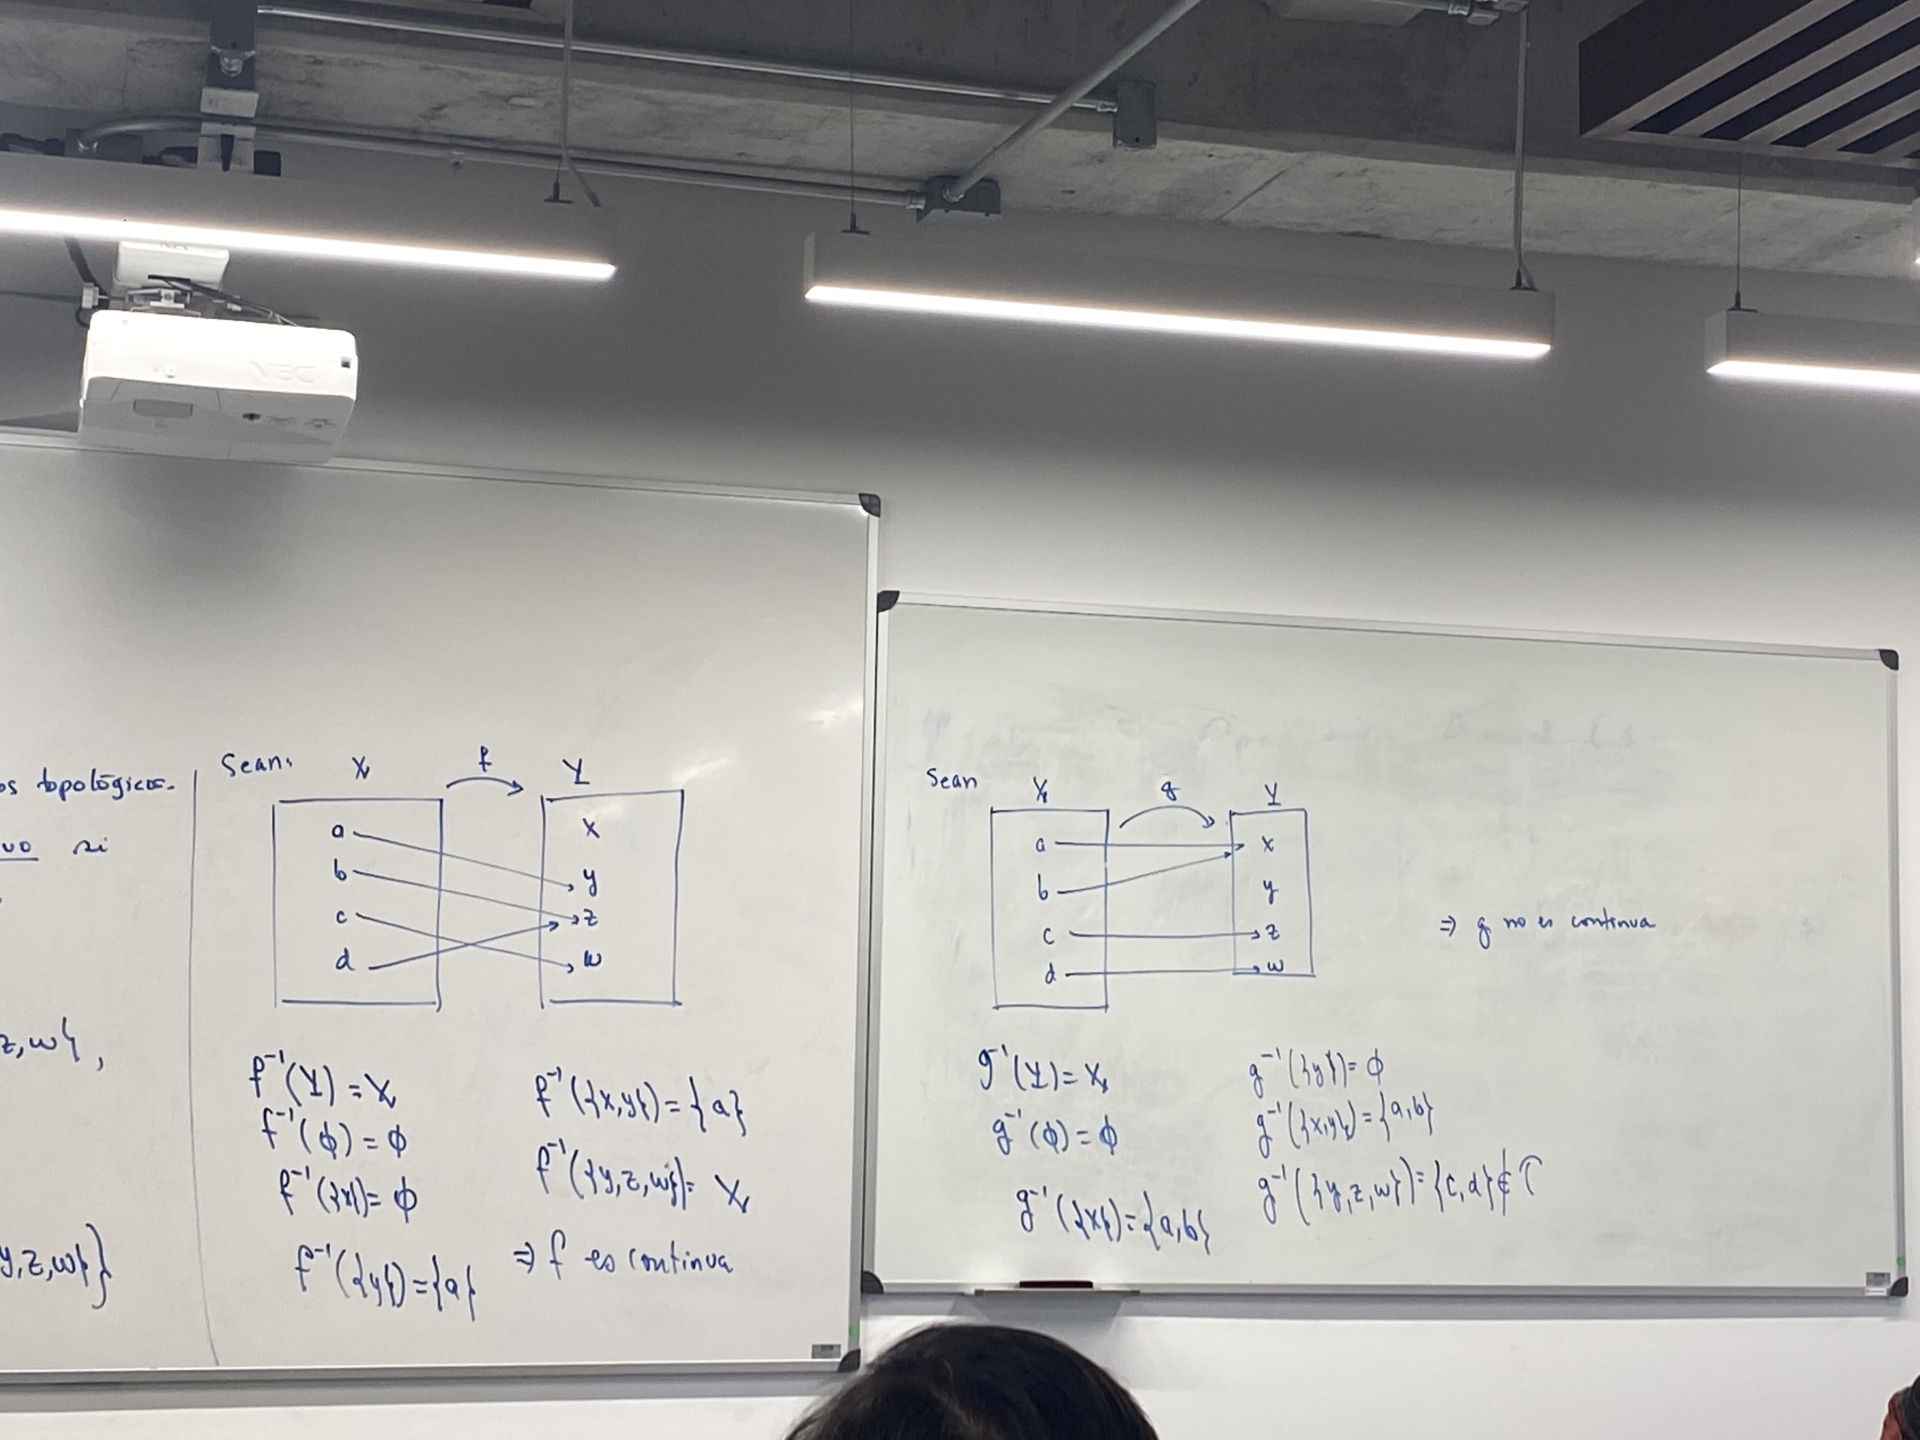
\includegraphics[scale=0.2]{imagenes/ejemplos1.jpeg}
    \end{figure}
\end{ejemplo}

\begin{nota}
    Sea $f: (X,\tau)\to (Y,\tau^*)$ un mapeo y suponga que $\beta=\{B_i\}$ es una base para $\tau^*$. Sea $G\in \tau^*\implies G=\bigcup_{i}B_i,B_i\in\beta $. Entonces, $f^{-1}(G)=g^{-1}\left(\bigcup_iB_i\right)=\bigcup_i f^{-1}(B_i)\implies f^{-1}(G)\in \tau$, si $f^{-1}(B_i)\in \tau$. 
\end{nota}

\begin{nota}
    Dado un mapeo $f:X\to Y$ y si $A\subseteq Y\implies f^{-1}[A^c]=[f^{-1}(A)]^c$. En efecto: Sea $x\in f^{-1}(A^c)\iff f(x)\in A^c \iff f(x)\not\in A\iff x\not\in f^{-1}(A)\iff x\in [f^{-1}(A)]^c$
    
\end{nota}

\begin{nota}
    \begin{enumerate}
        \item Sean $f:(X,\tau)\to(Y,\tau^*)$ un mapeo continuo y sea $F$ un cerrado de $Y\implies f^{-1}(F^c)=\left[f^{-1}(F)\right]^c\in \tau \implies f^{-1}(F)$ es cerrado en $X$.  
        \item Sea $G$ un abierto de $Y\implies G^c$ es cerrado de $Y$. Si $f^{-1}[G^c]=[f^{-1}(G)]^c$ es cerrado, entonces $f^{-1}(G)\in \tau\implies f$ es continuo 
    \end{enumerate}
    
\end{nota}


\begin{prop}
    Sea $f:X\to Y$ un mapeo entre espacios topológicos. Entonces, $f$ es un mapeo continuo ssi $f(\overline{A})\subset \overline{f(A)},\forall A\subseteq X$
    \begin{cajita}
        Propiedades: 
        \begin{enumerate}
            \item $f[f^{-1}(A)]=A$
            \item $f^{-1}[\underbrace{f(A)}_{\subseteq X}]\supset A$
        \end{enumerate}
    \end{cajita}
    \begin{dem}
        Sea
        \begin{itemize}
            \item $(\implies )$ Suponga que $f$ es continuo y sabemos que $f(A)\subset \overline{f(A)}\implies f^{-1}[f(A)]\subset f^{-1}[\overline{f(A)}]$. Además, como $\overline{f(A)}$ es cerrado $\implies f^{-1}[\overline{f(A)}]$ es cerrado (ya que $f$ continuo). Entonces, 
            \begin{align*}
                A\subseteq \underbrace{f^{-1}[\overline{A}]}_{cerrado} &\implies A\subset \overline{A}\subset f^{-1}[\overline{f(A)}]\\
                &\implies f(\overline{A})\subset f[f^{-1}[\overline{f(A)}]]\\
                &\implies f(\overline{A})\subset \overline{f(A)}
            \end{align*}
            \item $(\impliedby)$ Supóngase que $f(\overline{A})\subset \overline{f(A)},\forall A\subseteq X$. Sea $C$ un cerrado de $Y$. Sea $A=f^{-1}(C)\implies f[\overline{f^{-1}(C)}]\subseteq \overline{f(f^{-1}(C))}\implies f[\overline{f^{-1}(C)}]\subseteq C\implies f^{-1}[f[\overline{f^{-1}(C)}]]\subseteq f^{-1}(C)\implies \overline{f^{-1}(C)}\subset f^{-1}(C)\implies f^{-1}(C)\subset \overline{f^{-1}(C)}\subset f^{-1}(C)\implies f^{-1}(C)=\overline{f^{-1}(C)}\implies f^{-1}(C)$ es cerrado. 
        \end{itemize}
    \end{dem}
\end{prop}

\begin{prop}
    Sea $\{\tau_i\}$ una colección de topologías sobre $X$. Si $f:X\to Y$ es continuo con respecto a cada $\tau_i\implies f$ es continuo con respecto a $\tau=\bigcap_i\tau_i\implies f$ es continuo respecto a $\tau=\bigcap_i \tau_i$.
    \begin{dem}
        Sea $G$ un abierto de $Y\implies f^{-1}(G)\in \tau_i$ para cada $i$. Entonces, $f^{-1}(G)\in \bigcap_i\tau_i=\tau\implies f$ es continua con respecto a $\tau$. 
    \end{dem}
\end{prop}

\begin{prop}
    Sea $f:(X,\tau)\to (Y,\tau)$ un mapeo continuo, si $A\subset X\implies f|_A:(A,\tau_A)\to (Y,\tau')$ es continua. 
    \begin{dem}
        Como $f$ es continua $\implies$ si $G\in \tau'\implies f^{-1}\in \tau\implies A\cap f^{-1}(G)\in \tau_A\implies f|_A$ es continua (respecto a $\tau_A$). 
    \end{dem}
\end{prop} 
\begin{ejemplo}
    No se tomo bien la foto :(
\end{ejemplo}

\begin{ejemplo}
    Sea $f:(X,\tau)\to (X,\tau')$ tal que $\tau' =\{Y,\varnothing\}$. Entonces, $f^{-1}(Y)=X$ y $f^{-1}(Y)=X$ y $f^{-1}(\varnothing)=\varnothing\in \tau\implies f$ es continua, independientemente de $\tau$. 
\end{ejemplo}


\begin{ejemplo}
    Sea $f:(X,\tau)\to (Y,\tau')$, tal que: $\tau=P(X)\implies$ si $G\in \tau'\implies f^{-1}(G)\in P(X)\implies f$ es continua (para cada topologia $\tau'$). 
\end{ejemplo}

\begin{ejemplo}
    Considere el mapeo identidad 
    $$i:(X,\tau)\to (X,\tau')$$
    $\implies$ si $G\in\tau'\implies f^{-1}(G)=G\in \tau$. 
\end{ejemplo}

\begin{cajita}
    Continuidad local $\tau'\subset \tau$. 
\end{cajita}

\begin{definicion}
    Sean $(X,\tau)$ un espacio topológico y $x\in X$ un subconjunto $U\subseteq X$ es vecindad de $x$, si $\exists V\in \tau\ni x\in V\subset U$ (es decir, $x$ es un punto interior de $U$.)
\end{definicion}

\begin{definicion}
    Lqa colección de todas las vecindades de un punto $x\in X$ se llamna sistema de vecindades de $x$. Notación: $N_x$. 
\end{definicion}
\begin{prop}
    $N_x$ es cerrado bajo intersecciones y extensiones. Es decir: 
    \begin{enumerate}
        \item Si $u,w\in N_x\implies u\cap w\in N_x$.
        \item Si $u\in N_x$ y $u\subseteq w \implies w\in N_x$. 
    \end{enumerate}
        \begin{dem}
            Sea
            \begin{enumerate}
                \item Si $u\in N_x\implies \exists$ abierto $G\ni x\in G\subset u$. Si $w\in N_x\implies \exists$ abierto $H\ni x\in H\subset w\implies x\in G\cap H\subseteq u\cap w\implies u\cap w\in N_x$.
                \item Si $u\in N_x\implies \exists $ abierto $G\ni x\in G\subset u\subseteq w\implies w\in N_x$
            \end{enumerate}
            
        \end{dem}
\end{prop}
\begin{prop}
    Sea $A$ un subconjunto del espacio topológico $(X,\tau)\ni \forall x\in A\exists G\in\tau\ni x\in G\subset A$. Entonces, $A$ es abierto en $\tau$. 
\end{prop}
\begin{prop}
    Un conjunto $G$ es abierto ssi $G$ es vecindad de cada uno de sus puntos. 
    \begin{dem}
        Sea 
        \begin{enumerate}
            \item Prop. anterior. 
            \item Si $x\in G\implies \exists $ abierto $G\ni x\in G\subset G\implies G\in N_x,\forall x\in G$. 
        \end{enumerate}
    \end{dem}
\end{prop}

\begin{prop}
    Sea 
    \begin{enumerate}
        \item $N_x\neq \varnothing$ y $x\in A,\forall A\in N_x$. 
        \item Cada miembro $A\in N_x$ es un superconjunto de un miembro $G\in N_x$, donde $G$ es vecindad de cada uno de sus puntos. 
    \end{enumerate}
\end{prop}
\begin{definicion}
    Un mapeo $f:X\to Y$ entre espacios topologicos es continuo en un punto $x\in X$, para cada $U\in N_f(x)\exists V\in N_x\ni f(V)\subset U$. 
\end{definicion}

\begin{teorema}[Mala foto :(]
    Un mapeo $f:X\to Y$ entre espacios topologicos, es continuio ssi es continuo en cada punto de $X$. 
\end{teorema}
%---- 17-02
\begin{teorema}
    Un mapeo $f:X\to Y$ es continuo ssi es continuo en cada punto de $X$. 
    \begin{dem}
        Sea 
        \begin{itemize}
            \item Sea $f$ continua en cada punto de $X$ y sea $H$ un abierto en $Y$. A probar: $f^{-1}(H)$ es abierto en $X\iff f^{H}$ es vecindad de cada uno de sus puntos. 
            \item Sea $x\in f^{-1}(H) \implies f(x)\in H\implies H\in N_{f(x)}$. Por la continuidad de $f$ en $x\exists G\in N_x\ni f(G)\subset H\implies x\in G\subset f^{-1}[f(G)]\subset f^{-1}(H)$
        \end{itemize}
    \end{dem}
\end{teorema}

\begin{ejemplo}
    Sea $X=\{a,b,c,d\}$ y $\tau_1=\{X,\varnothing, \{a\},\{b\},\{a,b\},\{a,b,c\} \}$ y $\tau_2=\{X,\varnothing, \{a\},\{b\},\{a,b\},\{b,c,d\} \}$. Considere $f:X\to X$ tal que \begin{align*}
        a\to b\\
        b\to d\\
        c\to b\\
        d\to c
    \end{align*}
    Probar: 
    \begin{enumerate}
        \item $f$ es continua en $c$
        \item $f$ es continua en $d$. 
    \end{enumerate}
\end{ejemplo}

\begin{ejemplo}
    Sea $f:X\to Y$ y sea $\{p\}$ un abierto de $X$. 
    \begin{enumerate}
        \item Si $\{p\}$ es abierto, $\forall p\in X\implies$ la topologia de $X$ es la discreta $\implies f$ es continua. 
        \item Si $\{p\}$ es abierto, para algún $p\in X$. Sea $H\in N_{f(p)}\implies \exists \{p\}\in N_{f(p)}\implies \exists \{p\}\in N_p\ni f(\{p\})\subset H\implies f$ es continua en $p$. 
    \end{enumerate}
\end{ejemplo}
\begin{definicion}
    Una función $f:X\to Y$ es secuencialmente continua en un punto $p\in X$ ssi para cada sucesión $(a_n)$, se cumple que: si $a_n\to p\implies f(a_n)\to f(p)$
    \begin{cajita}
        Sea
        $$a_n\to p$$
        $\forall G$, abierto de $X\ni p\in G$, se tiene que $\exists N\in \mathbb{Z}^+\ni$ si $n\geq N\implies a_n\in G$. 
    \end{cajita}
\end{definicion}

\begin{teorema}
    Si una función $f:X\to Y$ es continua en $p\in X$, entonces $f$ es secuencialmente continua en $p\in X$. 
    \begin{sol}
        Sea 
        \begin{enumerate}
            \item Ejercicio. 
            \item Suponga quie $f$ es continua en $p\in X$ y que $(a_n)$, cumple: 
            $$a_n\to p$$
            A probar: $f(a_n)\to f(p)\iff \forall G$, abierto de $Y\ni f(p)\in G$, la cola de $f(a_n)$ esta en $G$. 
        \end{enumerate}
    \end{sol}
\end{teorema}
\begin{definicion}
    Un mapeo $f:X\to Y$ es 
    \begin{enumerate}
        \item Abierto, si $\forall G$, abierto de $X$, $f(G)$ es abierto de $Y$. 
        \item Cerrado, si $\forall H$, cerrado de $X$, $f(H)$ es cerrado de $Y$. 
    \end{enumerate}
\end{definicion}
\begin{ejemplo}
    Sea $f:\mathbb{R}\to \mathbb{R}\ni f(x)=1,\forall x\in \mathbb{R}$. Entonces, $f$ es continua. Sea $A\subseteq \mathbb{R}$. 
    \begin{enumerate}
        \item Si $A$ es abierto, entonces $f(A)=\{1\}\implies f$ no es abierta. 
        \item Si $A$ es cerrado $\implies f(A)=\{1\}$ es un cerrado $\implies f$ es cerrado. 
    \end{enumerate}
\end{ejemplo}

%---- 22-02
\begin{definicion}
    Los espacios topológicos $(X,\tau)$ y $(Y,\tau')$ son homeomorfos si existe una función $f:X\to Y$ tal que: 
    \begin{enumerate}
        \item $f$ es biyectiva. 
        \item $f$ y $f^{-1}$ son continuas.
    \end{enumerate}
    En este caso, $f$ es un homeomorfismo. 
\end{definicion}

\begin{nota}
    \begin{enumerate}
        \item Se dice que una función es bicontinua si es abierto y continua. 
        \item Un mapeo $f:X\to Y$ es un homeomorfismo ssi $f$ es bicontinuo y biyectivo.
    \end{enumerate}
    
\end{nota}

\begin{ejemplo}
    Sea $X=(-\pi/2,\pi/2)$ y sea $f: X\to \mathbb{R}$ tal que $f(x)=\tan x$. Note que: 
    \begin{enumerate}
        \item $f$ es biyectiva. 
        \item $f$ es continua y $f^{-1}(x)=\arctan x$ es continua. 
    \end{enumerate}
    Entocnes $f$ es un homeomorfismos. Tal que $(-\pi/2,\pi/2)$ y $R$ son homeomorfos. (topologicamente los mismos. )
\end{ejemplo}

\begin{nota}
    Una propiedad $p$ que comparten espacios topológicos homeomorfos es una invariante topológica.  
\end{nota}

\begin{ejemplo}
    La acotación no es una invariante topológica. 
\end{ejemplo}

\begin{ejemplo}
    Sea $D_1=\{(r,\theta)\ni |r|<1\}$ y $D_2=\{(r,\theta)\ni |r|<2\}$. Entonces, considere $f:D_1\to D_2\ni f(r,\theta)= (2r,\theta)$. Entonces, $f$ es un homeomorfismo entre $D_1$ y $D_2$. Note que el área no es un invariante topológico. 
\end{ejemplo}

\begin{ejemplo}
    Sean $(X,\tau_D)$ y $(Y,\tau_D)$ espacios discretos y sea $f:X\to Y$.
    Entonces $f$ es: \begin{enumerate}
        \item continua.
        \item abierta
    \end{enumerate}
    Entonces, es un homeomorfismo si comparten ccaardinalidad. 
\end{ejemplo}

\begin{nota} Sean
    \begin{enumerate}
        \item $X,Y,Z$ espacios topológicos. 
        \begin{nota}
            Notación: $X\approx Y $ significa $X$ es homeomorfo a $Y$. 
        \end{nota} 
        \begin{enumerate}
            \item $X\approx X,\forall X$
            \item Si $X\approx Y\implies Y \approx X$. 
            \item Si $X\approx Y$ y $Y\approx Z\implies X\approx Z$. 
        \end{enumerate}
        $\implies$ la relación $\approx$ es de equivalencia. (Implica que se produce una partición en el conjuntos de definición de la relación)
    \end{enumerate}
\end{nota}

\begin{prop}
    Sea $f:(X,\tau)\to (Y,\tau^*)$ un mapeo abierto e inyectivo y sea $A\subset X$ tal que $f(A)=B$. Entonces, la restricción $f_A:(A,\tau_A)\to (B,\tau_B)$
    es abierto e inyectivo. 
    \begin{dem}
        \begin{enumerate}
            \item La inyectividad se hereda. 
            \item A probar: $f$ es abierta, sea $H\in \tau_A\implies f(H)\in \tau_B^*$. Como $H\in \tau_A\implies \exists G\in \tau \ni G\cap A=H$. Tenemos \begin{align*}
                f(H) &= f(G\cap A)
                \intertext{Por la inyectividad:}
                &=f(G)\cap f(A)\\
                &= \underbrace{f(G)}_{\in \tau^*} \cap B\in \tau_B^*
            \end{align*} 
        \end{enumerate}
    \end{dem}  
\end{prop}

\begin{problema}
    Sea $\{(Y_i, \tau_i)\}$ una colección cualquiera de espacios topológicos, y para cada $i$ considere: 
    $$f_i: X\to Y_i$$
    donde $X$ es un conjunto no-vacío cualquiera. Encuentra la topología para $X\ni$ cada $f_i$ es continua. 
\end{problema}

%---- 24-02
\begin{teorema}
    Sea $\{f_i:X\to (Y_i,\tau_i)\}$ una colección de mapeos definidos sobre un conjunto vacio de $X$ sobre los espacios topologicos $(Y_i,\tau_i)$, sea 
    $$S=\bigcup_i \{f^{-1}(H):H\in \tau_i\},$$
    y definamos $\tau$ como la topologia sobre $X$ generada por $S$. 
    \begin{enumerate}
        \item Todos los $f_i$ son continuas con respecto a $\tau$. 
        \item Si $\tau^*$ es la intersección de todas las topologias sobre $X$ con respecto a las cuales las $f_i$ son continuas, entonces $\tau=\tau^*$. 
        \item $\tau$ es la topologia menos fina sobre $X$ tales que las $f_i$ son continuas. 
        \item $S$ es una subbase para $\tau$. 
    \end{enumerate}
\end{teorema}

\begin{ejemplo}
    Una función constante $f_i: X\to Y_i$ es continua con respecto a cada topologia sobre $X$. Entonces, todas las $f_i$ son continuas con respecto a la topologia indiscreta, es decir $\tau_i=\{X,\varnothing\}$. Note que $\tau_i$ es la topologia menos fina sobre $X\implies \tau_I$ es la topologia menos fina que hace continuas a las $f_i$. 
\end{ejemplo}

\begin{ejemplo}
    Sea $Y=\{a,b,c,d\}$ y la topologia sobre $Y$, $\tau=\{Y,\varnothing,\{c\},\{a,b,c\},\{c,d\}\}$. Considere $X=\{1,2,3,4\}$ y sean: $f:X\to (Y,\tau)$ y $g:X\to (Y,\tau)\ni $
    $$f:$$
    \begin{align*}
        1\to a\\
        2\to a\\
        3\to d\\
        4\to b 
    \end{align*}
    $$g:$$
    \begin{align*}
        1\to b\\
        2\to c\\
        3\to c\\
        4\to d
    \end{align*}
    Entonces, la topologia sobre $X$ que tiene menos abiertos y que hace continuos a $f$ y $g$, es la que tiene subbase: 
    $$S=\{f^{-1}(H):H\in \tau\}\bigcup \{g^{-1}(H):H\in\tau\}$$
    Entonces 
    $$S=\{X,\varnothing,\{1,2,4\},\{3\}\}\bigcup \{X,\varnothing,\{2,3\},\{1,2,3\},\{2,3,4\}\}$$
    Entonces,
    $$S=\{X,\varnothing,\{1,2,4\},\{3\}, \{2,3\},\{1,2,3\},\{2,3,4\}\}$$

\end{ejemplo}

\subsection*{Topologia producto}
Sea $X_\alpha$ un conjunto, $\forall \alpha \in I$. El producto cartesiano de las $x_\alpha$, es el conjunto 
$$\prod_{\alpha\in I} X_\alpha := \{x:I\to \bigcup_{\alpha\in I}X_\alpha \ni x(\alpha)\in X_\alpha, \forall \alpha \in I\}$$

\begin{ejemplo}
    Sea $I=\{1,2,3\}$ y sean $X_1=\{a,e\},X_2=\{o\},X_3=\{o,u\}$. Entonces 
    \begin{align*}
        x_1\times x_2\times x_3 &= \left\{x:\{1,2,3\}\to \bigcup_{i=1}^3 X_i\ni x(\alpha)\in X_\alpha\right\}\\
        &= \left\{x:\{1,2,3\}\to \{a,e,o,u\}: x(\alpha)\in X_\alpha\right\}
    \end{align*}
    Ademas 
    \begin{align*}
        x(1) = a\in X_1 \quad & x(1) = a\in X_1 & x(1) = e\in X_1 \quad& x(1) = e\in X_1\\
        x(2) = o\in X_2 \quad & x(2) = o\in X_2  & x(2) = o\in X_2  \quad& x(2) = o\in X_2\\
        x(3) = o\in X_3 \quad & x(3) = u\in X_3 & x(3) = o\in X_1  \quad& x(3) = u\in X_1\\
    \end{align*}
    Entonces 
    $$X_1\times X_2\times X_3=\{(a,o,o),(a,o,u),(e,o,o),(e,o,u)\}$$
\end{ejemplo}

\begin{ejemplo}
    $$
\begin{aligned}
&I=\{1,2\} \quad y \quad X=\{0,1\} \text {, entonces: } \\
& x \times x_1=x^2=\left\{x:\{1,2\} \rightarrow\{0,1\} \Rightarrow \begin{array}{rl}
x(\alpha) & \in x_{\alpha} \\
& \forall \alpha=1,2
\end{array}\right\} \\
& \begin{array}{l|l|l|l}
x(1)=0 & x(1)=1 & x(1)=0 & x(1)=1 \\
x(2)=0 & x(2)=1 & x(2)=1 & x(2)=0
\end{array} \\
& \Rightarrow x^2=\{(0,0),(1,1),(0,1),(1,0)\}
\end{aligned}
$$
\end{ejemplo}

\begin{ejemplo}
    Sea 
    $$
\begin{aligned}
& I=\mathbb{Z}^{+} \Rightarrow \prod_{\alpha \in I} X_\alpha=\left\{x: \mathbb{Z}^{+} \rightarrow \cup_{\alpha \in I} x_\alpha \exists x(\alpha)=x_{\alpha},\forall \alpha \in I\right\} \\
& =\left\{\left(x_1, x_2, \ldots\right): x(\alpha) \in x_\alpha, \forall \alpha \in \mathbb{Z}^{+}\right\}
\end{aligned}
$$
\end{ejemplo}
\begin{ejemplo}
    Si en al ejemplo anterior hacemos $X_\alpha=X$, sea $I$ un conjunta de indices cualquiera
$$
\begin{aligned}
& \Rightarrow \prod_{\alpha \in I} x_\alpha =\{x: I \rightarrow x: x(\alpha) \in x, \forall \alpha \in I\} \\
&=x^I
\end{aligned}
$$
\end{ejemplo}

\begin{problema}
    Sea $X_\alpha$ es un espacio topologica, $\forall \alpha\in I$. Se desea construir una topologia para $\prod_{\alpha\in I}\ni $
    \begin{enumerate}
        \item Esta topologia sea natural 
        \item Produzca suficientes teoremas de la forma: Si $x_\alpha$ tiene la propiedad $p,\forall \alpha \in I$. 
    \begin{figure}[H]
        \centering
        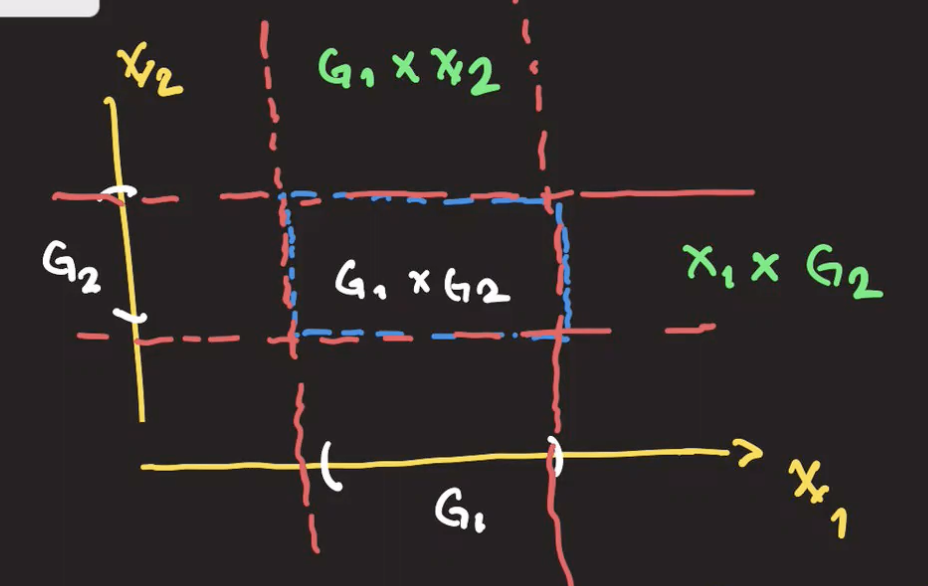
\includegraphics[scale=1]{imagenes/ejemplo2.png}
    \end{figure}
    $\implies G_1\times G_2=(G_1\times X_2)\cap (X_1\times G_2)$. Entonces, con dos espacios factor, los abiertos subbasicos serian las franjas $G_1\times X_2$ y $X_1\times G_2$. Entonces , en el caso de $n-$espacios factor, los abiertos subbasicos serian de la forma: 
    $$X_1\times X_2\times\cdots \times G_i\times X\cdots \times X_n$$
    \end{enumerate}
\end{problema}
\begin{cajita}
    Recordemos: Se define la $k$-Esima proyección $\pi_k$ cono el mapeo:
$$
\begin{aligned}
& \pi_K: \prod_{\alpha \in I} X_{\alpha} \longrightarrow X_{\alpha} \ni \\
& \pi_k(\omega) \longmapsto \omega_k \\
& \text { Ej: } \pi_2: \mathbb{R}^3 \longrightarrow \mathbb{R} \ni \\
& \pi_2\left(x_1, x_2, x_3\right)=x_2 \\
&
\end{aligned}
$$
\end{cajita}
\begin{definicion}
    Sea $\left\{x_\alpha \right\}_{\alpha \in I}$ una colección de espacios topológicos y sea $X=\prod_{\alpha \in I} x_\alpha$. La topologia menos fina que hace continuas a las proyecciones sobre $X$, es la topologia producto.
\end{definicion}

\begin{cajita}
    Si cada $X_\alpha$ es Hausdorff $\implies \prod_{\alpha\in I}X_\alpha$ es Hausdorff. 
\end{cajita}
%--- 01-03

\begin{definicion}
    Sean $(X_\alpha,\tau_\alpha)$, $\alpha\in I$ espacios topologicos y sea $X=\prod_{\alpha\in I}X_\alpha$
    \begin{enumerate}
        \item Las funciones $\pi_k:X\to X_k$ se llaman proyecciones.
        \item La topologia generada por las proyecciones en la topologia producto de $X$. 
        \item Es decir, es la topologia menos fuerte que hace continuas a las proyeccciones. 
        \item Un espacio producto tiene la forma $$\left(\prod_{\alpha\in I} X_\alpha,\tau\right)$$
    \end{enumerate}
\end{definicion}

\begin{prop}
    Sea $\{X_\alpha\}_{\alpha\in I}$ una colección de espacios de Hausdorff, y sea $X=\prod_\alpha X_\alpha$ el espacio producto. Entonces, $X$ es de Hausdorff. 
    \begin{dem}
        Sea $x,y\in X, x\neq y$. Entonces, $\exists k\ni$ los puntos $x$ y $y$ difieren en la $k$-esima coordenada. 
        $\pi_k:X\to X_k,$ produce las imagenes 
        $$pi_k(x)=x_k$$
        Y
        $$\pi_k(y)=y_k$$
        Como $x_k$ es Hausdorff, existen abiertos $G$ y $H$ de $x_k$ tal que $x_k\in G$, $y_k\in H$ y $G\cap H=\varnothing$. Entonces, $\pi_k^{-1}(G)$ y $\pi_k^{-1}(H)$ son abiertos de $X$, $x\in \pi_{k}^{-1}$, $y\in \pi_k^{-1}(H)$ y $\pi_k^{-1}(G)\cap \pi_{k}^{-1}(H)=\varnothing$ Entonces $X$ es Hausdorff. 
    \end{dem}
\end{prop}

\begin{cajita}
    Sea 
    \begin{enumerate}
        \item Topologia producto;
        $$S=\bigcup_\alpha \left\{\pi_\alpha^{-1}(u):u\in \tau_\alpha\right\}$$
        \item Por lo que los abiertos basicos tienen la forma: 
        \begin{align*}
            \pi_{k_1}^{-1}\left(G_{k_1}\right)\cap \pi_{k_2}^{-1}\left(G_{k_2}\right)\cap \cdots \cap \pi_{k_n}^{-1}\left(G_{k_n}\right)
        \end{align*}
        donde $G_{k_j}\in \tau_k$. 

        Ademas
        \begin{align*}
            \pi_i(G) = \begin{cases}
                \bigcap G_{i_\alpha}, k_n=1\\
                x_i,i\neq k_j, k=1,\cdots, n
            \end{cases}
        \end{align*}
    \end{enumerate}
\end{cajita}

\begin{problema}
    Una funcion $f$ del espacio topologico $\prod_\alpha X_\alpha$ es continua ssi para  cada proyeccion $\pi_i$, se tiene que $\pi_\alpha \circ f$ es continua. 
    \begin{dem}
        Sea 
        \begin{itemize}
            \item Como $f$ es continua y las $\pi_\alpha$ son continuas $\implies \pi_\alpha\circ f$ son continuas. 
            \item Sea $H$ un abierto en la topologia producto. A probar $f^{-1}(H)$ es abierto en $Y$. 
        \end{itemize}
    \end{dem}
\end{problema}

\begin{ejemplo}
    Sea $X=\mathbb{R}$, $I=\mathbb{R}$. Entonces
    $$\mathbb{R}^\mathbb{R}=\left\{f:\mathbb{R}\to \mathbb{R}\ni f(\alpha)\in \mathbb{R}\right\}$$
\end{ejemplo}

\begin{ejemplo}
    Sea $X=\mathbb{R}\implies I=\mathbb{Z}^+$. 
    $$\mathbb{R}^{\mathbb{Z}^+}=\{x:\mathbb{Z}^+ \to \mathbb{R}, x(m)\in \mathbb{R}_n\}$$
\end{ejemplo}

\subsection{Compactos}

\begin{definicion}
    Sea $(X,\tau)$ un espacio topológico una clase $\{H_i\}$ de abiertos de $X$ es una cubierta abierta de $X$, si $\bigcup_i H_i=X$. 
\end{definicion}

\begin{definicion}
    Una subclase de una cubierta abierta de $X$ que también es cubierta abierta es una subcubierta de la inicial. 
\end{definicion}
\begin{definicion}
    Un espacio compacto es un espacio topológico en el que cada cubierta abierta tiene una subcubierta finita. Es representar $X=\bigcup_{i\in I}^n H_i $
\end{definicion}

\begin{nota}
    Un subespacio compacto de $X$ es un subespacio que es compacto por derecho propio. 
\end{nota}

\begin{teorema}
    Todo subespacio cerrado de un espacio compacto es compacto.
    \begin{dem}
        Sea $F$ un cerrado de $X$ y considere el subespacio $(F,\tau_F)$. Sea $\{G_i\}$ una cubierta abierta de $F$, con $G_i\in \tau_F$. $G_i=F\cap H_i$, donde $H_i\in\tau$. Considere la cubierta abierta de $X:\{H_i\}\cup F^c$. Como $X$ es compacto, hay una subcubierta finita de la cubierta anterior: $\{H_{i_1},H_{i_2},H_{i_3},\cdots, H_{i_m}\}\cup F^c $. Entonces, tenemos $H_{i_j}\cap F=G_{ij}$, donde $h\subseteq \{G_{ij}\}$ son una subcubierta finita de $F$. 
    \end{dem} 
\end{teorema}

\begin{teorema}
    Cualquier imagen continua de un espacio compacto es compacto. 
    \begin{dem}
        Sea $(X,\tau)$ es un espacio topológico compacto y sea $(Y,\tau')$ y sea $f:X\to Y$ un mapeo continuo. A probar: $f(x)$ es compacto. Sea $\{G_i\}\subseteq  \tau'_{f(x)}$ una cubierta de $f(x)$, donde los $G_i$ son abiertos de $f(x)$ (topología relativa).
        \begin{cajita}
            Tenemos: 
        \begin{enumerate}
            \item $G_i=f(x)\cap \underbrace{H_i}_{\in \tau'}$
            \item $\bigcup G_i =f(x)$
        \end{enumerate}
        Entonces $f(x)\cap [\bigcup_i H_i]=f(x)$.Además, 
        \begin{align*}
            f(x) &\subset \bigcup_i H_i\\
            f^{-1}(f(x))& \subset f^{-1}(\bigcup_i H_i)\\
            x &\subset \bigcup_i f^{-1}(H_i)\\
            x&= \bigcup_{i=1}^m f^{-1}(H_i)\\
            f(x) &= \bigcup_{i=1}^{m}f(f^{-1}(H_i ))
        \end{align*}
        \end{cajita}
        
    \end{dem}
\end{teorema}

\begin{prop}
    Propiedad de intersección finita 
\end{prop}

\begin{teorema}
    Los enunciados siguientes son equivalentes: 
    \begin{enumerate}
        \item $X$ es un espacio compacto. 
        \item Para cada clase $\{F_i\}$ de cerrados de $X\ni \bigcap_{i}F_i=\varnothing$, se cumple que $\{F_i\}$ contiene una subclase finita $\{F_{i_1}, \cdots, F_{i_m}\}\ni F_{i_1}\cap \cdots \cap F_{i_m}=\varnothing$  
    \end{enumerate}
    \begin{dem}
        $(i)\implies (ii)$ Sea $X$ un espacio compacto y $\{F_i\}$ una clase de cerrados con $\{F_i\}\ni \bigcap_i F_i=\varnothing$. Entonces
        \begin{align*}
            X=\left(\bigcap_i F_i\right)^c = \bigcup_i F_i^c
        \end{align*}
        Entonces 
        $\{F_i^c\}$ es una cubierta abierta de $X$. Como $X$ es compacto, dicha cubierta tiene una subcubierta finita, $\{F_{i_1}^c,\cdots, F_{i_k}^c\}$, entonces 
        \begin{align*}
            X= \bigcup_{j=1}^k F_{i_j}^c 
        \end{align*}
        Entonces 
        $$\varnothing =F_{i_1}\cap \cdots \cap F_{i_k}$$

        $(ii)\implies (i)$ Sea $\{G_i\}$ una cubierta abierta de $X$. Entonces $\bigcup_i G_i = X\implies (\bigcup_i G_i)^c =X^c \implies \bigcap_i G_i^c=\varnothing$. Donde $\{G_i^c\}$ es la clase de cerrados. Entonces $\{G_i^c\}$ tiene una subclase finita: 
        $$\{G_{i_1}^c,\cdots, G_{i_m}^c\}\ni G_{i_1}^c\cap\cdots \cap G_{i_m}^c=\varnothing$$
        Por De Morgan, $G_{i_1}\cup \cdots \cup G_{i_m}=X$. Es decir que $\{G_{i_j}\}$ es una subcubierta finita para $X$. Entonces, $X$ es compacto. 
    \end{dem}
\end{teorema}

\begin{nota}
    Dada una clase de conjuntos $C=\{C_i\}$, se dice que $C$ tiene la propiedad de intersección finita $(Pif)$ si para cada $C_{i_1}, \cdots C_{i_k}$ se cumple $\bigcap_{j=1}^k C_{i_j}\neq \varnothing$.  
\end{nota}

\begin{ejemplo}
    Considere: 
    $$C=\{[1,\infty), [2,\infty), \cdots, [n, \infty),\cdots\}$$
    Considere $$C_1=[n,\infty),C_2=[n_2,\infty), \cdots, C_k=[n_k,\infty)$$
    Entonces 
    $$\bigcup_{i=1}^k C_i=[\max_{1\leq i\leq k}\{n_i\},\infty)\neq \varnothing$$ 
    Entonces $C$ tiene la pif. 
\end{ejemplo}

\begin{ejemplo}
    Sea $C=\{\left(-\frac{1}{n},\frac{1}{n}\right):n\in\mathbb{Z}^+\}$
    Entonces, $C_1=\left(-\frac{1}{n_1},\frac{1}{n_1}\right),C_2=\left(-\frac{1}{n_2},\frac{1}{n_2}\right)\cdots C_k=\left(-\frac{1}{n_k},\frac{1}{n_k}\right)$. 
    Entonces 
    $$\bigcap_{i=1}^k\left(-\frac{1}{n_i},\frac{1}{n_i}\right) = \left(-\frac{1}{\max\{n_i\}},\frac{1}{\max\{n_i\}}\right) $$
    Entonces, $C$ tiene la pif. 
\end{ejemplo}
\begin{nota}
    En el teorema anterior, la contrapuesta de $(ii)$ es para toda clase de cerrados de $X$, $\{F_i\}$ tal que cada subclase finita tiene intersección no vacía, entonces $\bigcap_i F_i\neq \varnothing$. Es decir, cada clase de cerrados de $X$ que tiene la pif, tiene intersección no vacía. 
\end{nota}

\begin{teorema}
    $X$ es un espacio compacto ssi cadad clase de cerrados de $X$ que tiene la pif, tinee intersección no vacía. 
\end{teorema}


\begin{teorema}
    Un espacio topológico es compacto si cada cubierta abierta básica tiene subcubierta abierta finita. 
    \begin{dem}
        Sea $\{G_i\}$ una cubierta abierta del espacio topológico $X$ y sea $\{B_i\}$ una base para $X$. Sabemos que cada $G_i$ es unión de algunos $B_j$, es decir $\{B_j\}$ es uan cubierta abierta («básica») de $X$. Por hipótesis, $\{B_j\}$ tiene una subcubierta finita. Tomemos, para cada miembro de la subcubierta, un $G_i$ que lo contenga. Entonces, $X$ es compacto. 
    \end{dem}
\end{teorema}

\begin{teorema}
    Un espacio topológico es compacto si cada cubierta abierta subbásica tiene una subcubierta finita. 
\end{teorema}

\begin{teorema}
    En un espacio de $T_2$, cualquier punto y un subespacio disjunto y compacto, puede separarse por abiertos, en el sentido que tienen vecindades disjuntas. 
    \begin{figure}[H]
        \centering
        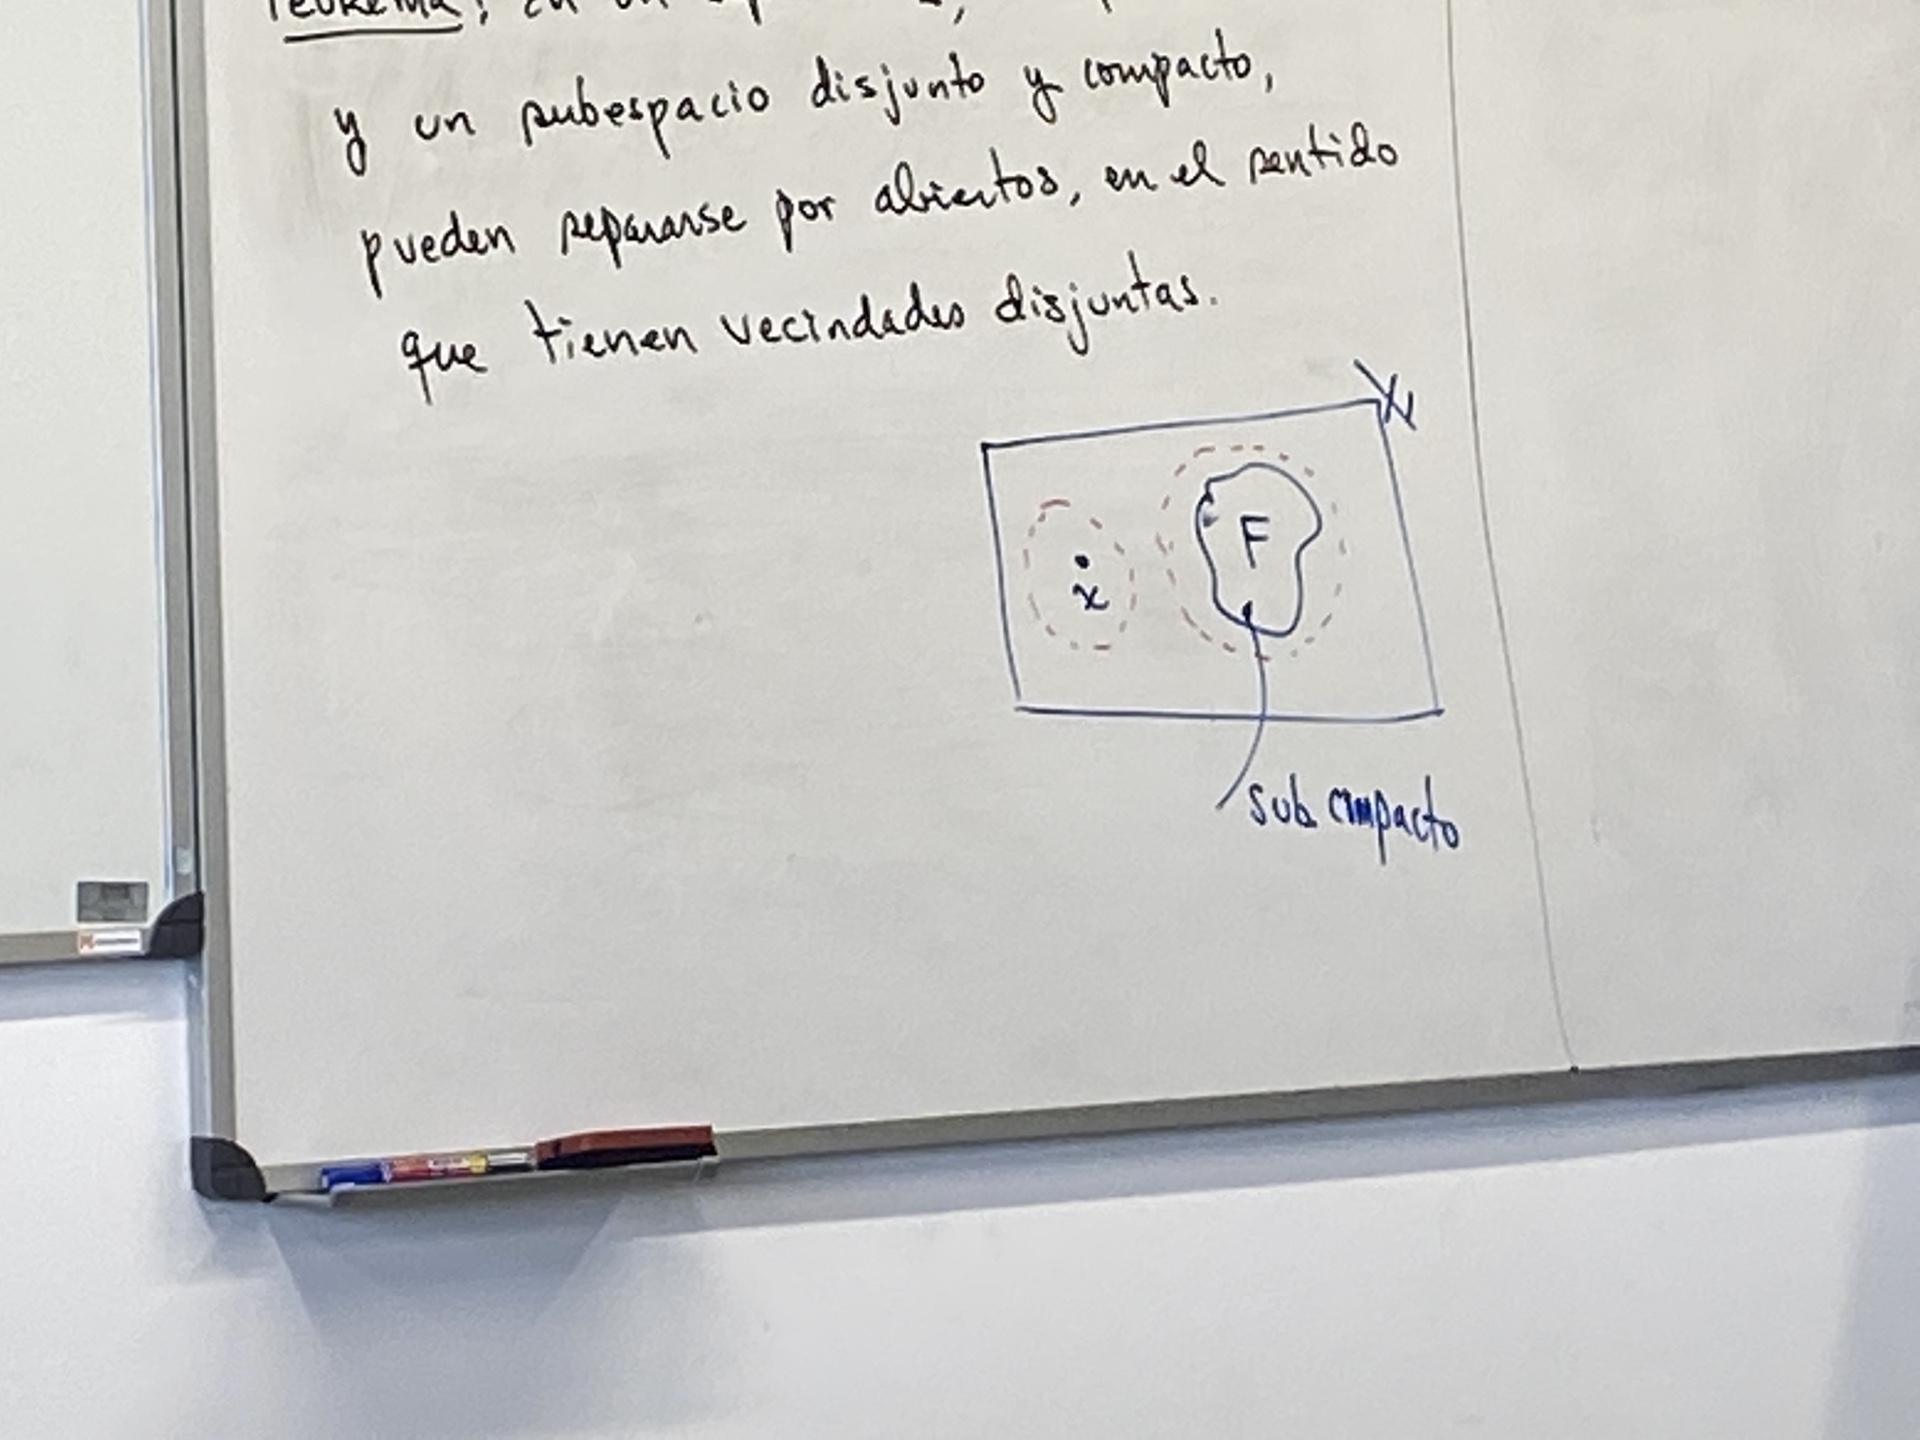
\includegraphics[scale=0.1]{imagenes/ejemplo3.jpeg}
    \end{figure}
    \begin{dem}
        Sea $x\in X$ y sea $F$ un subesapcio compacto de $X$ tal que $x\not\in F$. Sea $y\in F\implies$ Como $X$ es $T_2$, existen vecindades disjuntas $G_y$ y $H_y$ tal que $x\in G_y, y\in H_y$, $G_x\cap H_y=\varnothing$. Variando y sobre todo $F$, se tiene que $\bigcup_y H_y$ es una cubierta abierta de $F$. Como $F$ es compacto, existe una subcubierta finita de $F$, digamos: 
        $$F\subset H_{y_1}\cup H_{y_2}\cup\cdots \cup H_{y_k}=H$$
        y considere la vecindad de $X$, $G=G_{y_1}\cap G_{y_2}\cap\cdots \cap G_{y_k}$
        Nótese que $G$ y $H$ son disjuntos. 
    \end{dem}
\end{teorema}

\begin{teorema}
    Cada subespacio compacto de un $T_2$ es cerrado. 
    \begin{dem}
        Sea $X$ un $T_2$ y $F$ un subespacio compacto de $X$. A probar: $F^c$ es abierto. 
        \begin{enumerate}
            \item Que $F^c=\varnothing'\implies $ es abierto. 
            \item Supóngase que $F^c\neq \varnothing\implies$ sea $x\in F^c$. Por el teorema anterior, existen vecindades disjuntas $G_x$ y $H_F$, es decir $x\in G_x\subset F^c\implies F^c$ es abierto, entonces $F$ es cerrado.   
        \end{enumerate}
    \end{dem}
\end{teorema}

\begin{teorema}
    Un mapeo biyectivo y continuo de un espacio compacto en un espacio de Hausdorff es un homeomorfismo. 
\end{teorema}


\begin{definicion}
    Un espacio $X$ es $T_1$ si, para $x,y\in X$, $x\neq y$, existen vecindades $G$ y $H$ tales que $x\in G$ y $y\not\in G$; $y\in H$ y $x\not\in H$ 
\end{definicion}

\begin{teorema}
    Un espacio topológico es $T_1$ ssi los unitarios son cerrados. 
    \begin{dem}
        Sea $x\in X$ y sea $\{x\}$ un cerrado de $X\iff \{x\}^c$ es un abierto $\iff$ si $y\neq x$, $y$ tiene una vecindad que no contiene a $x\iff X$ es $T_1$. 
    \end{dem}
\end{teorema}

\begin{prop}
    Tenemos 
    \begin{enumerate}
        \item $\mathbb{R}$ con la topología usual es $T_1$. 
        \item Cada $T_2$ es $T_1$. 
    \end{enumerate}
\end{prop}

\begin{ejemplo}
    Encuentre un espacio $T_1$ que no es $T_2$. $\mathbb{R}$ con la topología cofinita. 
\end{ejemplo}
\begin{ejemplo}
    Sea $X=\{a,b\}$ y $\tau=\{X,\varnothing, \{
        a\}\}$ entonces $(X,T)$ no es $T_1$. 
\end{ejemplo}

\begin{teorema}
    Cada subespacio de un $T_1$ es un $T_1$. 
    \begin{dem}
        Sea $A$ un subespacio de $(X,\tau)$. Sean $x,y\in A,x\neq y $
        \begin{itemize}
            \item Como $x,y\in A\subset X\implies \exists G,H\in \tau\ni x\in G, y\not\in G, x\not\in H, y\in H$. 
            \item A probar: si $x\in A\implies \{x\}$ es cerrado de $\tau_A\iff \{x\}^c =A-\{x\}$ es abierto de $\tau_A$. Entonces, $(\underbrace{X-\{x\}}_{\in\tau})\cap A = A-\{x\}\in \tau_A\implies A-\left[A-\{x\}\right]$ es un cerrado, que implica que es igual a $\{x\}$
        \end{itemize}
    \end{dem}
\end{teorema}

\begin{nota}
    Un subconjunto finito de un $T_1$ no tiene puntos límite. Considere el conjunto finito $\{a_1,a_2,\cdots,a_n\}$ en $X$, el cual también es cerrado. Tomemos ahora, $\{a_2,a_3,\cdots,a_n\}$, el cual es cerrado. Esto implica que $\{a_2,a_3\cdots,a_n\}^c$ es un abierto. Note que $a_1\in \{a_2,a_3,\cdots,a_n\}^c$
\end{nota}

\begin{definicion}
    Un espacio $X$ es regular ssi satisface: 
    si $F$ es un cerrado de $X$ y $p\in X\ni p\not\in F$, existen abiertos $G$ y $G\ni F\subset G$ y $\{p\}\subset H$. $G\cap H=\varnothing$
\end{definicion}

\begin{nota}
    Sean $X=\{a,b,c\}$ y $\tau=\{X,\varnothing, \{a\},\{b,c\}\}$ los cerrados de $X$ son: $X,\varnothing,\{b,c\},\{a\}$. Nótese que $\{b\}$ no es cerrado $\implies X$ no es $T_1$, además, $X$ es regular.  
\end{nota}

\begin{definicion}
    Un espacio topológico es $T_3$ si es regular y $T_1$. 
\end{definicion}

\begin{teorema}
    Si $X$ es $T_3$ entonces $X$ es $T_2$. 
    \begin{dem}
        Sean $x,y\in X, x\neq y$. Entonces, $\{x\}$ es cerrado, ya que $X$ es $T_1$. Como $X$ es regular, existen vecindades disjuntas $G$ y $H\ni x\in \{X\}\subset G$ y $y\in H$, $G\cap H =\varnothing\implies X$ es un $T_2$.  
    \end{dem}
\end{teorema}

\begin{teorema}
    Un espacio $X$ es normal es normal si para $F_1$ y $F_2$, cerrados disjuntos de $X$, existen vecindades dijuntas $G$ y $H$ tal que $F_1\subset G$ y $F_2\subset H$.
\end{teorema}

\begin{ejemplo}
    Sea $X=\{a,b,c\}$ y $\tau=\{X,\varnothing, \{a\}, \{b\}, \{a,b\}\}$ los cerrados son: $\varnothing,X,\{b,c\},\{a,c\},\{c\}$. Como $\{a\}$ no es cerrado entonces $X$ no es $T_1$ y $X$ no es normal. 
\end{ejemplo}

\begin{definicion}
    Un espacio topológico que es normal y $T_1$ es un $T_4$. 
\end{definicion}

\begin{teorema}
    Los enunciados siguientes son equivalentes: 
    \begin{enumerate}
        \item $X$ es normal 
        \item Si $H$ es un superconjunto abierto del cerrado $F$, existe un abierto $G$ tal que 
        $$F\subset G\subset \overline{G}\subset H$$
    \end{enumerate}
    \begin{dem}
        Sea
        \begin{itemize}
            \item $(\impliedby)$ Sean $F_1$ y $F_2$ cerrados disjuntos de $X$. Entonces, existen un abierto $G\ni F_1\subset G\subset \overline{G}\subset F_2^c$. Entonces, como $\overline{G}\subset F_2^c\implies (F_2^c)^c\subset (\overline{G})^c\implies F_2\subset (\overline{G})^c$ (aabierto, disjunto de $G$)
            \item Sea $X$ normal, $F$ un cerrado de y $H$ un superconjunto abierto de $F$. Nótese que $H^c$ es un cerrado disjunto de $F\implies$ existen abiertos $G$ y $L\ni G\subset G$ y $H^c \subset L\implies L^c\subset H$, además: $F\subset G,L^c\subset H$. $G\subset L^c\implies F\subset G\subset \overline{G}\subset H$. 
        \end{itemize}
    \end{dem}
\end{teorema}

\begin{prop}
    Si $X$ es un $T_4\implies X$ es un $T_3$.
\end{prop}

\begin{dem}
    Como $X$ es $T_4\implies X$ es normal y $T_1$. A probar: $X$ es regular. Sean $x\in X$ y $F$ es un cerrado de $X\ni x\not\in F\implies \{x\}$ es un cerrado disjunto de $F\implies $ existen abiertos disjuntos $G$ y $H\ni x\in \{x\}\subset G$ y $F\subset H\implies X$ es regular.   
\end{dem}